\documentclass[10pt]{article}
\usepackage[utf8]{inputenc}
\usepackage[T1]{fontenc}
\usepackage{amsmath}
\usepackage{amsfonts}
\usepackage{amssymb}
\usepackage[version=4]{mhchem}
\usepackage{stmaryrd}
\usepackage{graphicx}
\usepackage[export]{adjustbox}
\graphicspath{ {./images/} }

\begin{document}

    During the radiation dominated era in the early Universe, the scale factor of the Universe $a \propto t^{1 / 2}$, where $t$ is the time since Big Bang. During most of this era, neutrons ( n ) and protons ( p ) remain in thermal equilibrium with each other via weak interactions. The number density ( $N$ ) of free neutrons or protons is related to the temperature $T$ and their corresponding masses $m$ such that

    $$
    N \propto m^{3 / 2} \exp \left(-\frac{m c^{2}}{k_{\mathrm{B}} T}\right),
    $$
    
    as long as time $t \leq t_{\mathrm{wk}}=1.70 \mathrm{~s}$, when $k_{\mathrm{B}} T \geq k_{\mathrm{B}} T_{\mathrm{wk}}=800 \mathrm{keV}$. After $t_{\mathrm{wk}}$, the weak interactions can no longer maintain such equilibrium, and free neutrons decay to protons with a half-life time of 610.4 s .\\
    (T10.1) Let the number density of protons be $N_{\mathrm{p}}$, and that of neutrons be $N_{\mathrm{n}}$. Calculate the relative abundance of neutrons given by the ratio $X_{\mathrm{n}, \mathrm{wk}}=N_{\mathrm{n}} /\left(N_{\mathrm{n}}+N_{\mathrm{p}}\right)$ at time $t_{\mathrm{wk}}$.\\
    (T10.2) Photons maintain thermal equilibrium and retain a blackbody spectrum at all epochs.\\
    (T10.2a) Find the index $\beta$, such that $T(a) \propto a^{\beta}$.\\
    (T10.2b) Identify which of the following graphs shows the correct behaviour of the spectral energy density for two temperatures $T_{1}$ and $T_{2}$. Tick $(\checkmark)$ the correct option in the Summary Answersheet.\\
    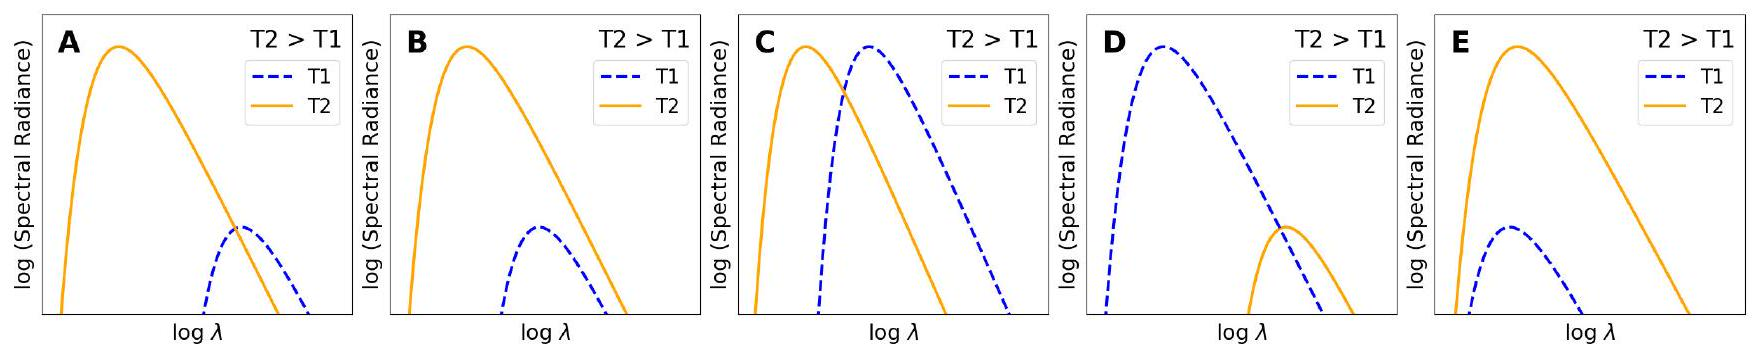
\includegraphics[max width=\textwidth, center]{2025_08_23_e94579452776a99c4850g-12}\\
    (T10.3) After $t_{\mathrm{wk}}$, the process of formation of deuterium from protons and neutrons is governed by the Saha equation, given by the Indian physicist Prof. Meghnad Saha, which can be simplified to
    
    $$
    \frac{N_{\mathrm{D}}}{N_{\mathrm{n}}}=6.5 \eta\left(\frac{k_{\mathrm{B}} T}{m_{\mathrm{n}} c^{2}}\right)^{3 / 2} \exp \left(-\frac{\left(m_{\mathrm{D}}-m_{\mathrm{p}}-m_{\mathrm{n}}\right) c^{2}}{k_{\mathrm{B}} T}\right) .
    $$
    
    Here, baryon-to-photon ratio $\eta$ is $6.1 \times 10^{-10}$, and $N_{\mathrm{D}}$ is the number density of deuterium.\\
    (T10.3a) Plot the ratio $N_{\mathrm{D}} / N_{\mathrm{n}}$ on the grid in the Summary Answersheet, for at least 4 reasonably spaced values of temperature that lie in the domain $k_{\mathrm{B}} T=[60,70] \mathrm{keV}$, and draw a smooth curve passing through these points.\\
    (T10.3b) From the plot find $k_{\mathrm{B}} T_{\text {nuc }}$ (in keV) when $N_{\mathrm{D}}=N_{\mathrm{n}}$.\\
    (T10.3c) Instead, now assume that all the free neutrons combine instantaneously with the protons at $k_{\mathrm{B}} T_{\text {nuc }}$ to form Deuterium, and all of which immediately gets converted to Helium $\left({ }_{2}^{4} \mathrm{He}\right)$. Compute the corresponding epoch or time of nucleosynthesis, $t_{\mathrm{nuc}}(\mathrm{in} \mathrm{s})$, for the formation of Helium.\\
    (T10.4) Calculate the value of $X_{\mathrm{n} \text {, nuc }}$ immediately before $t_{\mathrm{nuc}}$.\\
    (T10.5) The primordial Helium abundance, $Y_{\text {prim }}$, is defined to be the fraction of total baryonic mass in the Universe that is bound in Helium just after $t_{\text {nuc }}$. Obtain a theoretical estimate for the value of $Y_{\text {prim }}$ . For the purpose of this calculation alone, assume $m_{\mathrm{p}} \approx m_{\mathrm{n}}$ and that the mass of Helium, $m_{\mathrm{He}} \approx 4 m_{\mathrm{n}}$.\\
    (T10.6) The primordial abundance of Helium is very difficult to measure, as stars continuously convert Hydrogen to Helium in the Universe. The amount of processing by stars in a galaxy is characterised by the relative number density of Oxygen (which is only produced by stars) to hydrogen, denoted as $(\mathrm{O} / \mathrm{H})$, in the galaxy. A compilation of the measurements of $(\mathrm{O} / \mathrm{H})$ and the Helium abundance, $Y$, for different galaxies is plotted below.\\
    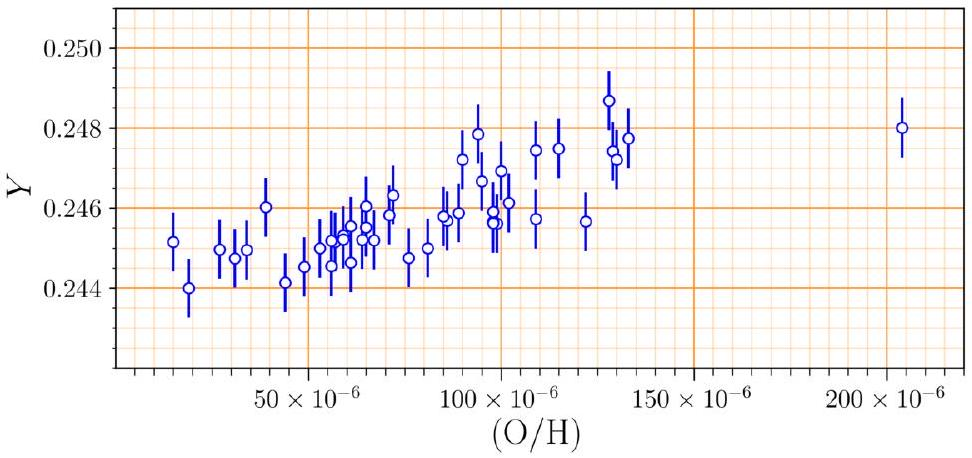
\includegraphics[max width=\textwidth, center]{2025_08_23_e94579452776a99c4850g-13}
    
    Use all of the points in this plot (which is reproduced in the Summary Answersheet) to answer the following.\\
    (T10.6a) Estimate $Y$ for a blue compact dwarf galaxy with a value of $(\mathrm{O} / \mathrm{H})=1.75 \times 10^{-4}$.\\
    (T10.6b) Obtain the slope $d Y / d(\mathrm{O} / \mathrm{H})$ of the straight line fit to the above data.\\
    (T10.6c) Estimate the primordial Helium abundance, $Y_{\text {prim }}^{\text {obs }}$, based on the above observations.\\
    (T10.7) The deviation between $Y_{\text {prim }}$ and $Y_{\text {prim }}^{\text {obs }}$ can be reconciled by changing the baryon-to-photon ratio $\eta$. When $\eta$ is decreased, as indicated by $\downarrow$ in the Summary Answersheet, indicate the increase ( $\uparrow$ ) or decrease ( $\downarrow$ ) in $N_{\mathrm{D}} / N_{\mathrm{n}}(T), T_{\text {nuc }}$ (when $N_{\mathrm{D}}=N_{\mathrm{n}}$ ), $t_{\text {nuc }}, X_{\mathrm{n} \text {, nuc }}$, and $Y_{\text {prim }}$ in the boxes provided in the Summary Answersheet.
    
\end{document}